\documentclass[conference,a4paper]{IEEEtran}
\IEEEoverridecommandlockouts
% ============================================================
% Paquetes
% ============================================================
\usepackage[utf8]{inputenc}
\usepackage[T1]{fontenc}
\usepackage[spanish,es-tabla]{babel}
\usepackage{amsmath,amssymb,amsfonts}
\usepackage{graphicx}
\usepackage{textcomp}
\usepackage{xcolor}
\usepackage{booktabs}
\usepackage{multirow}
\usepackage{array}
\usepackage{float}
\usepackage{cite}

\graphicspath{{../figs/etapas/}{../chapters/chapter3/Sections/Research Questions/sections/RQ2/img/}}

% Cambios de la versión extendida (respuesta a los Revisores #3, #4 y #5).
% \marcarcambiosfalse -> versión limpia (formato IEEE, texto en negro).
% \marcarcambiostrue  -> texto nuevo o modificado en azul, como en el Word del tutor.
% El texto íntegro del Word (sin condensar, ~10 páginas) está en paper_jcc2026_extendida_completa.tex.
\newif\ifmarcarcambios
\marcarcambiosfalse
\definecolor{azulcambio}{HTML}{1155CC}
\newcommand{\cambio}[1]{\ifmarcarcambios\ifvmode\leavevmode\fi{\color{azulcambio}#1}\else#1\fi}

% Traducción segura de "Index Terms" (no falla si la macro no existe en la instalación)
\makeatletter
\@ifundefined{IEEEkeywordsname}{\newcommand{\IEEEkeywordsname}{Palabras Clave}}{\renewcommand{\IEEEkeywordsname}{Palabras Clave}}
\makeatother

\begin{document}

% Título del tutor (Word, en inglés): "Benefit of Class Balancing Is Metric-Dependent:
% Feature Selection and Software Defect Prediction Evidence from BugHunter".
% Se traduce al español por la regla del JCC2026 (trabajos en español).
\title{\cambio{El Beneficio del Balanceo de Clases Depende de la Métrica: Evidencia sobre Selección de Características y Predicción de Defectos de Software en BugHunter}}

% ------------------------------------------------------------------
% Formato de autores IEEE (plantilla oficial):
%   línea 1: Nombre Apellido        <- sin grados académicos (Dr., Ph.D.)
%   línea 2: departamento (cursiva)
%   línea 3: institución (cursiva)
%   línea 4: Ciudad, País
%   línea 5: correo electrónico u ORCID
% ------------------------------------------------------------------
% \and separa los bloques y los distribuye en columnas (3 autores = 3 columnas).
% El nombre del departamento se corta a mano para que las 3 columnas quepan
% lado a lado sin desbordar el ancho de página.
\author{
\IEEEauthorblockN{1\textsuperscript{er} Jordanys Rodríguez Wong}
\IEEEauthorblockA{\textit{Depto. de Ingeniería de} \\
\textit{Sistemas y Computación} \\
\textit{Universidad Católica del Norte} \\
Antofagasta, Chile \\
jordanys.rodriguez@ce.ucn.cl}
\and
\IEEEauthorblockN{2\textsuperscript{do} Claudio Meneses Villegas}
\IEEEauthorblockA{\textit{Depto. de Ingeniería de} \\
\textit{Sistemas y Computación} \\
\textit{Universidad Católica del Norte} \\
Antofagasta, Chile \\
cmeneses@ucn.cl}      % <-- VERIFICAR correo institucional
\and
\IEEEauthorblockN{3\textsuperscript{er} Jaime Pavlich-Mariscal}
\IEEEauthorblockA{\textit{Depto. de Ingeniería de} \\
\textit{Sistemas} \\
\textit{Pontificia Universidad Javeriana} \\
Bogotá, Colombia \\
jaime.pavlich@gmail.com}   % <-- VERIFICAR correo institucional (afiliación según Word del tutor)
}

\maketitle

\begin{abstract}
La predicción de defectos de software enfrenta dos retos persistentes: alta dimensionalidad y desequilibrio de clases. Este trabajo evalúa si un preprocesamiento en dos etapas, selección de características por análisis de relevancia y control de redundancia seguida de balanceo de clases, mejora la predicción sobre BugHunter, un dataset de 15 proyectos Java con métricas en tres niveles de granularidad (archivo, clase, método). Se aplican Ganancia de Información, Chi-Cuadrado y ReliefF para relevancia; Incertidumbre Simétrica y Semejanza de Coseno para redundancia; ROS, RUS y SMOTE para balanceo; y Random Forest, XGBoost y SVM lineal como clasificadores, totalizando 42.356 ejecuciones. La selección de características reduce la dimensionalidad \cambio{(reducción mediana de 40\,\%, 88\,\% y 50\,\% de las métricas en los niveles de método, clase y archivo, y hasta un 94\,\% en el mejor caso individual)} con pérdida de \textit{F-measure} inferior a 0,02, y las métricas de tamaño de código (CLOC, LOC, LLOC) son los predictores más consistentes. El hallazgo más relevante concierne al balanceo: aplicado solo al entrenamiento, no mejora el \textit{F-measure} ponderado cuando el conjunto de prueba conserva la distribución real (prueba de Wilcoxon pareada con tamaño de efecto de Cliff insignificante), pero sí mejora de forma consistente la detección de la clase minoritaria (\textit{F-measure} de la clase \textit{bug} y MCC) en los tres clasificadores, un beneficio que la métrica agregada enmascara. Entrenar por proyecto individual supera sistemáticamente al conjunto unificado. \cambio{La conclusión sobre la utilidad del balanceo depende, por tanto, críticamente de la métrica de evaluación empleada.}
\end{abstract}

\begin{IEEEkeywords}
predicción de defectos de software, selección de características, desequilibrio de clases, BugHunter, Random Forest, MCC, reconocimiento de patrones
\end{IEEEkeywords}

\section{Introducción}

El software se integra en cada vez más ámbitos de la vida cotidiana, lo que exige mantener altos estándares de calidad en todo su ciclo de vida. Las fallas no detectadas durante las pruebas pueden derivar en transacciones defectuosas, interrupciones de servicio y fallas en cascada sobre sistemas dependientes \cite{singh2024,ferenc2020}. La Predicción de Fallas de Software (PFS) busca anticipar estos problemas identificando, antes de la fase de pruebas, los elementos de código con mayor probabilidad de contener errores.

Durante años, la escasez de conjuntos de datos públicos dificultó comparar métodos de PFS. Repositorios como PROMISE \cite{promise2005}, inspirado en el de la UCI \cite{uci1987}, y conjuntos como NASA, SOFTLAB, ReLink, AEEEM y Eclipse paliaron este problema, aunque la mayoría se limita a métricas de tamaño y complejidad capturadas en pocas versiones de lanzamiento. Ferenc et al. \cite{ferenc2020} propusieron capturar el estado del código inmediatamente antes y después de cada corrección de error en 15 proyectos Java de GitHub, dando origen a BugHunter, con métricas en tres niveles de granularidad (archivo, clase y método).

La calidad de estos conjuntos condiciona el desempeño de los modelos de predicción \cite{rathi2023}; entre sus problemas más señalados están la alta dimensionalidad, producto de características poco relevantes o redundantes, y el desequilibrio de clases \cite{tantithamthavorn2020}. Este trabajo aborda ambos sobre BugHunter mediante (i) selección de características en dos etapas, combinando análisis de relevancia y control de redundancia, y (ii) balanceo del conjunto de entrenamiento mediante \textit{Random Over-Sampling} (ROS), \textit{Random Under-Sampling} (RUS) y \textit{Synthetic Minority Over-sampling Technique} (SMOTE). Tomando como línea base la réplica de \cite{ferenc2020} con Random Forest en Weka, se responden cinco preguntas de investigación:

\begin{itemize}
\item \textbf{RQ1.} \textquestiondown{}El análisis de relevancia y el control de redundancia de características mejoran la identificación de errores basada en métricas de código?
\item \textbf{RQ2.} \textquestiondown{}Qué métricas de código son mejores predictoras de errores y en qué nivel de granularidad ofrecen mejores resultados?
\item \textbf{RQ3.} \textquestiondown{}Cómo influye la variación de los parámetros de los algoritmos de relevancia y redundancia en los resultados de clasificación?
\item \textbf{RQ4.} \textquestiondown{}Cómo influyen los algoritmos de balanceo de clases ROS, RUS y SMOTE en los resultados de los clasificadores?
\item \textbf{RQ5.} \textquestiondown{}Qué diferencias existen entre entrenar con el conjunto unificado de proyectos y entrenar con cada proyecto por separado?
\end{itemize}

La contribución principal es una evaluación experimental de 13.916 ejecuciones de Random Forest, complementada por un análisis de sensibilidad de 28.440 ejecuciones con XGBoost y SVM lineal, que identifica las métricas de código más relevantes, cuantifica el efecto del balanceo cuando el conjunto de prueba conserva su distribución original (incluido su efecto sobre las métricas por clase) y compara el entrenamiento por proyecto individual frente al conjunto unificado. \cambio{Además, se explicita el orden de las etapas de preprocesamiento respecto de la partición entrenamiento/prueba, se advierten los sesgos de selección post-hoc en RQ1 y RQ2, y se declara como trabajo futuro la validación con selección de características anidada y validación cruzada repetida (Secciones \ref{sec:metodologia}, \ref{sec:amenazas} y \ref{sec:conclusiones}).}

\section{Trabajos Relacionados}

BugHunter \cite{ferenc2020} se diferencia de conjuntos tradicionales como PROMISE o Eclipse \cite{promise2005} porque captura métricas en el instante más cercano a la introducción y corrección de cada error, en lugar de comparar versiones de lanzamiento completas; sus métricas se extraen con OpenStaticAnalyzer \cite{osa2004} en tres niveles de granularidad. Singh y Thankachan \cite{singh2021survey} revisan los marcos de aprendizaje automático aplicados a la PFS, y Li et al. \cite{li2018} señalan el desequilibrio de clases y la alta dimensionalidad como sus principales desafíos abiertos.

Liu et al. \cite{liu2015} y Chen et al. \cite{chen2013} propusieron el marco en dos etapas que se adopta aquí: un análisis de relevancia (Ganancia de Información, Chi-Cuadrado, ReliefF) seguido de un control de redundancia por agrupamiento por umbral (\textit{Neighbor-based Threshold Clustering}, NTC), con Incertidumbre Simétrica \cite{yu2003} o Semejanza de Coseno como medida de similitud. \cambio{Estos trabajos, al igual que el presente estudio, calculan la selección sobre el conjunto completo antes de particionar entrenamiento y prueba, una práctica común en PFS cuya implicancia se discute en las Secciones \ref{sec:seleccion} y \ref{sec:amenazas}.} Sobre el desequilibrio, Tantithamthavorn et al. \cite{tantithamthavorn2020} muestran que el efecto del rebalanceo depende fuertemente del contexto experimental, y Rathi et al. \cite{rathi2023} y Hossen et al. \cite{hossen2020} reportan mejoras al combinar muestreo y selección de características sobre proyectos de PROMISE. El presente trabajo evalúa dicha combinación sobre BugHunter, compara los tres niveles de granularidad y contrasta el entrenamiento por proyecto frente al conjunto unificado (RQ5), un análisis no cubierto por esos estudios.

Una línea más reciente sustituye las métricas por representaciones profundas del código: redes neuronales de grafos sobre el árbol de sintaxis abstracta (AST) \cite{sikic2022}, la combinación de la semántica de cada archivo (CNN sobre el AST) con las dependencias entre clases (GCN) \cite{zhou2022}, su extensión semisupervisada mediante destilación de conocimiento \cite{liu2024sedpgk}, la localización de defectos a nivel de línea \cite{pornprasit2023} y codificaciones semántico-sintácticas del AST para la transferencia entre proyectos, donde la heterogeneidad de distribuciones sigue siendo el principal obstáculo \cite{jiang2024}. En predicción \textit{just-in-time}, Guo et al. \cite{guo2023} reportan mejoras con seis modelos preentrenados de código, donde el balance de los datos de entrenamiento resulta determinante con pocos datos, y el benchmark ReDef \cite{nam2026} muestra que la calidad de las etiquetas condiciona las conclusiones sobre estos modelos. Las revisiones de Giray et al. \cite{giray2023} y de Stradowski y Madeyski \cite{stradowski2023} coinciden en que estos modelos elevan el costo computacional sin superar de forma consistente a los clasificadores clásicos sobre métricas tabulares, y señalan la brecha con su adopción industrial; los modelos de lenguaje de gran escala (LLM) abren, además, una nueva agenda \cite{hou2024,fan2023} que incluye la detección de defectos \cite{chen2026llm}. Frente a estos enfoques, que requieren el código fuente completo y cómputo considerable, las métricas tabulares con clasificadores clásicos conservan un bajo costo e interpretabilidad, y aportan líneas base rigurosas para evaluar si las representaciones profundas mejoran realmente.

\section{Conjunto de Datos y Metodología}
\label{sec:metodologia}

\subsection{BugHunter}

BugHunter \cite{ferenc2020} se construyó automáticamente a partir de 15 proyectos Java de GitHub, seleccionados por su tamaño, dominio y cantidad de errores reportados. A diferencia de los conjuntos tradicionales, que caracterizan todos los elementos de código de una versión de lanzamiento, captura el estado de cada elemento (archivo, clase o método) justo antes de detectarse un error y justo después de su corrección, e ignora los elementos nunca afectados por errores. Sus métricas, extraídas con OpenStaticAnalyzer \cite{osa2004}, cubren tamaño, complejidad, cohesión, acoplamiento, clonación de código y violaciones de reglas de codificación (\textit{code smells}): 72 a nivel de método, 92 a nivel de clase y 6 a nivel de archivo, además de un conjunto ``All'' por nivel que une los 15 proyectos.

La Tabla \ref{tab:desbalance} resume la distribución de clases de los 45 conjuntos proyecto-nivel tras binarizar el atributo \textit{Number of Bugs}. El desequilibrio es moderado frente a conjuntos clásicos de PFS como NASA o PROMISE, donde la clase con error suele representar menos del 10\,\% de las instancias \cite{tantithamthavorn2020}: la mediana de instancias \textit{bug} es del 28,1\,\%, 41,1\,\% y 42,7\,\% a nivel de método, clase y archivo, y en \textit{hazelcast}, \textit{MapDB} y \textit{elasticsearch} la clase \textit{bug} llega a ser mayoritaria a nivel de archivo. Esto es consecuencia de que BugHunter solo incluye elementos afectados por errores, y acota el sesgo de las métricas agregadas hacia la clase mayoritaria (Sección \ref{sec:amenazas}). El caso más desequilibrado es \textit{oryx} (razón no-bug:bug de 7,6:1 a nivel de método), lo que debe considerarse al interpretar su desempeño, el más alto del estudio.

\begin{table}[H]
\caption{Proporción de instancias con error (\textit{bug}) por nivel de granularidad, sobre los 15 proyectos individuales}
\label{tab:desbalance}
\centering
\resizebox{\columnwidth}{!}{%
\begin{tabular}{lccccc}
\toprule
Nivel & Mediana & Mín. (proyecto) & Máx. (proyecto) & ``All'' & Razón mediana \\
      & \% bug  & \% bug          & \% bug          & \% bug  & no-bug:bug \\
\midrule
Método  & 28,1 & 11,7 (\textit{oryx}) & 42,2 (\textit{hazelcast}) & 37,0 & 2,6:1 \\
Clase   & 41,1 & 12,5 (\textit{oryx}) & 53,0 (\textit{hazelcast}) & 48,6 & 1,4:1 \\
Archivo & 42,7 & 13,2 (\textit{oryx}) & 55,2 (\textit{hazelcast}) & 50,7 & 1,3:1 \\
\bottomrule
\end{tabular}}
\end{table}

\subsection{Selección de características en dos etapas}
\label{sec:seleccion}

Siguiendo a Liu et al. \cite{liu2015}, la selección de características se ejecuta en dos etapas.

\textit{Análisis de relevancia.} La importancia de cada característica se calcula con Ganancia de Información (IG), Chi-Cuadrado (CS) y ReliefF (RF). IG mide la reducción de entropía al dividir el conjunto de datos según una característica,
\begin{equation}
H = -\sum_{x} p(x)\log_{2}p(x),
\label{eq:entropia}
\end{equation}
donde $p(x)$ es la probabilidad de que una instancia pertenezca a la clase $x$. CS compara la distribución observada de una característica con la esperada bajo independencia respecto a la clase,
\begin{equation}
\chi^{2} = \sum \frac{(O-E)^{2}}{E}.
\label{eq:chisqr}
\end{equation}
ReliefF actualiza el peso $W[A]$ de cada característica $A$ comparando instancias muestreadas al azar con su vecino más cercano de la misma clase (\textit{hit}, $H$) y de la clase contraria (\textit{miss}, $M$),
\begin{equation}
W[A] = W[A] - \frac{\mathrm{diff}(A,R,H)}{m} + \frac{\mathrm{diff}(A,R,M)}{m},
\label{eq:relief}
\end{equation}
donde $R$ es la instancia muestreada, $\mathrm{diff}(\cdot)$ la diferencia normalizada en $A$ y $m$ el número de muestreos. En cada caso se conservan las $k$ características cuyo ranking supera un umbral relativo (\textit{Rank} $\in \{0{,}5, 0{,}7, 0{,}9\}$).

\textit{Control de redundancia.} Sobre el subconjunto resultante se aplica NTC \cite{liu2015}, que construye un grafo de vecino más cercano entre características y descarta aquellas cuya similitud con otra ya seleccionada supera un umbral $\beta \in \{0{,}5, 0{,}7, 0{,}9\}$. La similitud se mide con Incertidumbre Simétrica (SU),
\begin{equation}
SU(X,Y) = 2 \times \frac{I(X;Y)}{H(X)+H(Y)},
\label{eq:su}
\end{equation}
donde $I(X;Y)$ es la información mutua entre las dos características \cite{yu2003}, o con Semejanza de Coseno (COS) entre sus vectores de valores. Combinar los tres algoritmos de relevancia con las dos medidas de redundancia produce seis esquemas: IG\_SU, CS\_SU, RF\_SU, IG\_COS, CS\_COS y RF\_COS.

\cambio{\textit{Orden de las etapas respecto de la partición entrenamiento/prueba.} La relevancia y la redundancia se calculan sobre el conjunto proyecto-nivel completo, antes de la partición descrita en la Sección \ref{sec:diseno}, mientras que el balanceo (Sección \ref{sec:balanceo}) se aplica exclusivamente dentro del entrenamiento. Como IG, CS y RF utilizan la etiqueta de clase, este orden introduce un riesgo de sesgo de selección (\textit{selection bias}): el subconjunto elegido puede estar influido por instancias que luego integrarán el conjunto de prueba \cite{ambroise2002,cawley2010}. El riesgo afecta solo la elección de qué columnas conservar, no los parámetros del clasificador, que se ajustan exclusivamente sobre el entrenamiento. Su magnitud se discute en la Sección \ref{sec:amenazas}, y su corrección mediante una selección anidada, recalculada dentro de cada partición de entrenamiento, se declara como trabajo futuro (Sección \ref{sec:conclusiones}).}

\subsection{Balanceo de clases}
\label{sec:balanceo}

Sobre el entrenamiento ya filtrado se aplican, de forma independiente, tres técnicas de remuestreo \cite{junsomboon2017,hossen2020}: RUS elimina al azar instancias de la clase mayoritaria; ROS duplica al azar instancias de la clase minoritaria; y SMOTE genera instancias sintéticas de la clase minoritaria interpolando entre una instancia real y uno de sus $k$ vecinos más cercanos,
\begin{equation}
x_{\text{nueva}} = x_{i} + (x_{\text{vecino}} - x_{i}) \times r, \quad r \in [0,1].
\label{eq:smote}
\end{equation}
El conjunto de prueba conserva siempre la distribución original de clases, para que el rendimiento reportado no quede sobreestimado por instancias artificiales.

\subsection{Clasificador y diseño experimental}
\label{sec:diseno}

Se emplea Random Forest (RF) \cite{shah2020}, un ensamble de árboles de decisión entrenados sobre subconjuntos aleatorios de instancias y características (\textit{bagging}) que combina el voto de todos los árboles. La línea base se ejecuta en Weka \cite{weka2005} y el resto de los experimentos en Python (\textit{scikit-learn}).

En el \textbf{Paso 1} (selección), cada conjunto proyecto-nivel se recorre variando \textit{Rank} y $\beta$ para obtener el subconjunto de métricas de cada esquema. En el \textbf{Paso 2} (clasificación), el conjunto filtrado se divide en 67\,\% de entrenamiento y 33\,\% de prueba con muestreo estratificado; el entrenamiento, original o balanceado con ROS, RUS o SMOTE, se evalúa contra el mismo conjunto de prueba. El flujo se repite para los 15 proyectos y ``All'' en los tres niveles: la línea base (sin selección) requirió 2.592 ejecuciones y el estudio de selección y balanceo, 13.916 ejecuciones de RF. El desempeño se mide con precisión, \textit{recall} y \textit{F-measure}:
\begin{equation}
P = \frac{TP}{TP+FP}, \quad R = \frac{TP}{TP+FN}, \quad F_{1} = \frac{2PR}{P+R}.
\label{eq:pr}
\end{equation}
Se reporta el \textit{F-measure} agregado, ponderado por la frecuencia de cada clase. De las 13.916 ejecuciones solo se almacenaron métricas agregadas (precisión, \textit{recall}, \textit{F-measure} y exactitud) y parámetros de configuración, sin predicciones, matrices de confusión ni probabilidades; por ello, métricas más informativas bajo desequilibrio (\textit{F-measure} de la clase \textit{bug}, AUC-ROC y coeficiente de correlación de Matthews, MCC) no pueden recomputarse sin repetirlas, salvo en la línea base Weka de ``All'' a nivel de método, cuya salida completa se conservó (Sección \ref{sec:baseline}).

\textit{Análisis de sensibilidad.} Para mitigar dos amenazas del diseño anterior, el uso de un único clasificador y la diferencia de herramienta y esquema de validación entre la línea base y los experimentos, se repitió el flujo completo sobre los 48 conjuntos proyecto-nivel con tres clasificadores de paradigmas distintos: RF, XGBoost \cite{chen2016} (\textit{boosting} de gradiente) y una SVM lineal \cite{cortes1995} con estandarización previa. Los tres comparten la misma partición estratificada 67/33 en cada conjunto, lo que permite comparaciones pareadas; se reutilizan los subconjuntos del Paso 1, el balanceo se aplica solo al entrenamiento, y de cada una de las 28.440 ejecuciones (9.480 por clasificador) se almacenan las métricas agregadas y por clase (\textit{F-measure} de la clase \textit{bug}, MCC y AUC-ROC). Los resultados se reportan en la Sección \ref{sec:sensibilidad}.

\cambio{\textit{Sobre el uso de una semilla fija.} La semilla fija de la partición 67/33, en el estudio principal y en el análisis de sensibilidad, es una decisión deliberada: permite comparar esquemas de selección, técnicas de balanceo y clasificadores sobre exactamente la misma división de datos, habilitando las comparaciones pareadas de la Tabla \ref{tab:sensibilidad}. Implica, no obstante, que ninguno de los dos estudios promedia sobre múltiples particiones aleatorias, lo que se discute como amenaza a la validez (Sección \ref{sec:amenazas}) y se declara como trabajo futuro (Sección \ref{sec:conclusiones}).}

\section{Resultados Experimentales}

\subsection{Línea base}
\label{sec:baseline}

La Tabla \ref{tab:baseline} compara el \textit{F-measure} promedio de la réplica de Ferenc et al. \cite{ferenc2020} con solo Random Forest frente al reportado en el estudio original, que emplea once algoritmos. Los resultados son comparables, lo que valida a RF como base de comparación. Individualmente, \textit{oryx} obtuvo el mejor desempeño en los tres niveles (Tabla \ref{tab:oryx}, columna ``Original''), mientras que en \cite{ferenc2020} el mejor proyecto a nivel de método fue \textit{antlr4}, diferencia atribuible al uso de un único algoritmo de clasificación.

\begin{table}[H]
\caption{F-measure promedio: línea base replicada vs. \cite{ferenc2020}}
\label{tab:baseline}
\centering
\begin{tabular}{lcc}
\toprule
Nivel & Este trabajo & Ferenc et al. \cite{ferenc2020} \\
\midrule
Método  & 0,63 & 0,63 \\
Clase   & 0,50 & 0,56 \\
Archivo & 0,50 & 0,54 \\
\bottomrule
\end{tabular}
\end{table}

La salida completa conservada de la línea base del conjunto ``All'' a nivel de método permite desglosar su desempeño por clase (Tabla \ref{tab:porclase}): el \textit{F-measure} ponderado de 0,565 encubre un \textit{F-measure} de solo 0,356 para la clase \textit{bug} (precisión de 0,410 y \textit{recall} de 0,314), con un MCC de 0,052 y un AUC-ROC de 0,539, apenas superiores a los de un clasificador aleatorio. Este contraste cuantifica cuánto puede encubrir la métrica agregada respecto de la clase de interés práctico (Secciones \ref{sec:RQ4} y \ref{sec:amenazas}) y es coherente con el desempeño no superior del conjunto unificado (RQ5).

\begin{table}[H]
\caption{Desglose por clase de la línea base (Weka, Random Forest, validación cruzada de 10 particiones) sobre el conjunto ``All'' a nivel de método}
\label{tab:porclase}
\centering
\resizebox{\columnwidth}{!}{%
\begin{tabular}{lccccc}
\toprule
Clase & Precisión & \textit{Recall} & \textit{F-measure} & MCC & AUC-ROC \\
\midrule
No-bug & 0,646 & 0,735 & 0,688 & \multirow{2}{*}{0,052} & \multirow{2}{*}{0,539} \\
Bug    & 0,410 & 0,314 & 0,356 &  &  \\
\midrule
Prom. ponderado & 0,559 & 0,579 & 0,565 & 0,052 & 0,539 \\
\bottomrule
\end{tabular}}
\end{table}

\subsection{RQ1: efecto de la selección de características}
\label{sec:RQ1}

La Tabla \ref{tab:oryx} resume, para el proyecto con mejor desempeño (\textit{oryx}), el número de métricas y el \textit{F-measure} antes y después de aplicar el mejor esquema de selección, con entrenamiento sin balancear y balanceado. La selección redujo la dimensionalidad entre un 48,9\,\% y un 94,4\,\% con un \textit{F-measure} prácticamente equivalente a la línea base (diferencias de entre $-0{,}014$ y $+0{,}036$). El patrón se confirma sobre los 15 proyectos individuales (Tabla \ref{tab:agg}): la mediana del mejor \textit{F-measure} apenas varía entre las versiones sin balancear y balanceada, con reducciones medianas de características del 40\,\%, 88\,\% y 50\,\% a nivel de método, clase y archivo.

\cambio{\textit{Advertencia sobre el sesgo de comparar el mejor esquema contra una única referencia.} Las Tablas \ref{tab:oryx}, \ref{tab:agg} y \ref{tab:sensibilidad} comparan el mejor esquema de selección, i.e., un máximo sobre 54 combinaciones de algoritmo de relevancia, medida de redundancia, \textit{Rank} y $\beta$, frente a una única configuración de referencia (todas las características). Esto introduce una asimetría optimista estructural, análoga a la discutida para RQ4 (Sección \ref{sec:RQ4}), pero que, a diferencia de aquella, no se cancela mediante una comparación simétrica. Por ello, la evidencia más robusta de RQ1 son las medianas (reducciones de 40\,\%, 88\,\% y 50\,\% sin balanceo en la Tabla \ref{tab:agg}, y de 31\,\%--82\,\% en la Sección \ref{sec:sensibilidad}), con un \textit{F-measure} comparable a la línea base, y no el máximo de 94\,\% de una única celda (\textit{oryx}, nivel método). Eliminar esta asimetría, seleccionando el esquema sobre una partición de validación independiente de la de prueba, se declara como trabajo futuro (Sección \ref{sec:conclusiones}).}

\begin{table}[H]
\caption{Mejor resultado por nivel (proyecto \textit{oryx}): características originales vs. seleccionadas}
\label{tab:oryx}
\centering
\resizebox{\columnwidth}{!}{%
\begin{tabular}{lcccc}
\toprule
Nivel & Original (métr. / F) & Sel. sin balancear & Sel. balanceado & Reducción \\
\midrule
Método  & 72 / 0,852 & 29 métr. / 0,838 & 4 métr. / 0,837  & 59,7\,\% / 94,4\,\% \\
Clase   & 92 / 0,787 & 6 métr. / 0,786  & 47 métr. / 0,780 & 93,5\,\% / 48,9\,\% \\
Archivo & 6 / 0,770  & 3 métr. / 0,806  & 3 métr. / 0,777  & 50,0\,\% / 50,0\,\% \\
\bottomrule
\end{tabular}}
\end{table}

\begin{table}[H]
\caption{Mejor \textit{F-measure} por proyecto agregado sobre los 15 proyectos individuales (mediana [mín--máx])}
\label{tab:agg}
\centering
\resizebox{\columnwidth}{!}{%
\begin{tabular}{lcc}
\toprule
Nivel & Sin balancear & Balanceado \\
\midrule
Método  & 0,620 [0,538--0,838] & 0,615 [0,525--0,837] \\
Clase   & 0,524 [0,448--0,786] & 0,519 [0,460--0,780] \\
Archivo & 0,525 [0,456--0,806] & 0,547 [0,436--0,777] \\
\bottomrule
\end{tabular}}
\end{table}

La Semejanza de Coseno (COS) predominó en el control de redundancia a nivel de método y archivo, y la Incertidumbre Simétrica (SU) a nivel de clase. En conjunto, el análisis de relevancia y el control de redundancia reducen drásticamente las métricas necesarias sin comprometer la capacidad predictiva del modelo.

\subsection{RQ2: métricas más relevantes}
\label{sec:RQ2}

Al ordenar las métricas por su frecuencia de selección en los seis esquemas (Fig. \ref{fig:frecuencia}), CLOC, LOC y LLOC, las únicas tres disponibles en los tres niveles de granularidad, se ubicaron entre las más seleccionadas, lo que sugiere que las métricas de tamaño de código aportan un valor predictivo consistente en todos los niveles. Las métricas de nivel de método fueron las más seleccionadas, seguidas por las de clase y archivo. Las métricas de clonación mostraron aportes relevantes, mientras que las de violación de reglas de codificación (\textit{code smells}), salvo TNOS, presentaron muy baja variación y rara vez fueron seleccionadas.

\begin{figure}[H]
\centering
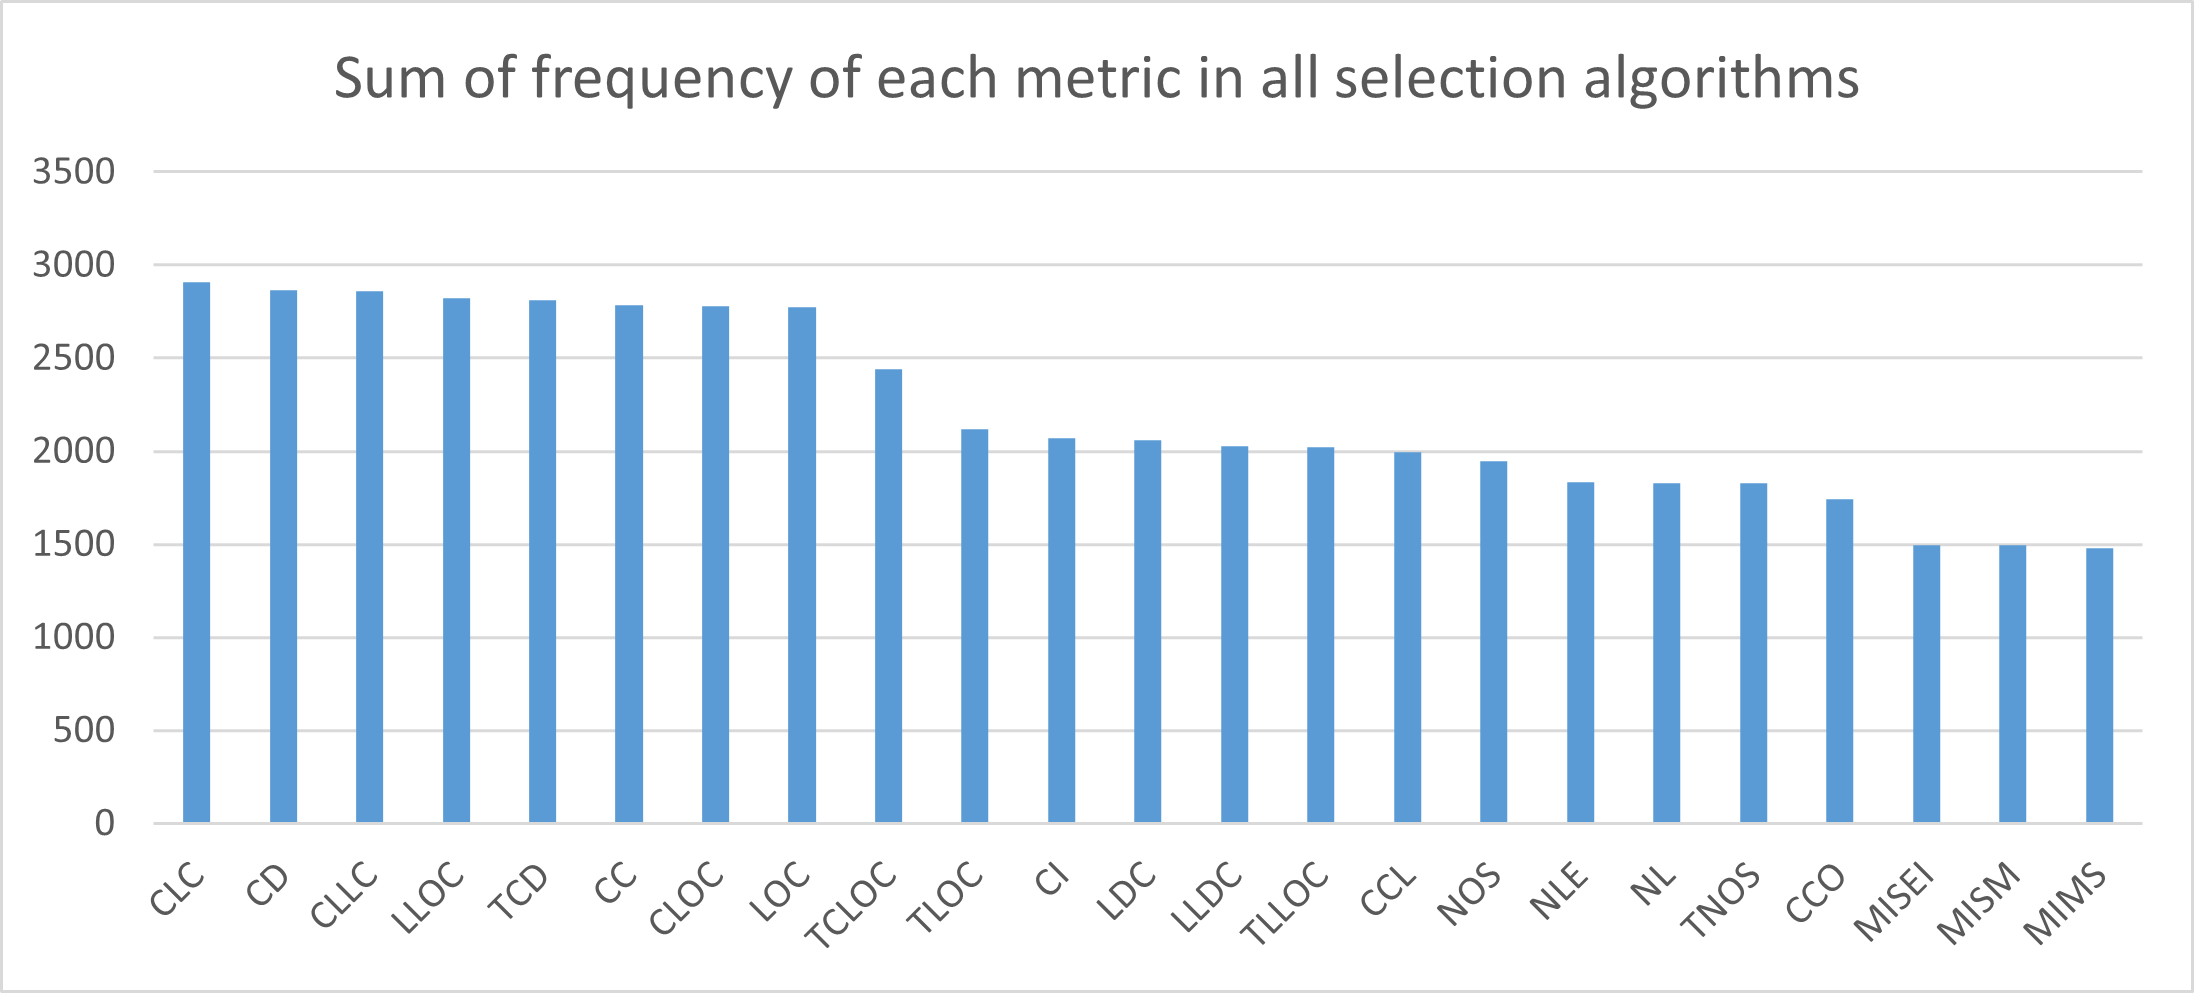
\includegraphics[width=0.95\columnwidth]{frec_all.png}
\caption{Frecuencia de selección de las métricas de código a través de los seis esquemas de selección de características.}
\label{fig:frecuencia}
\end{figure}

\cambio{\textit{Advertencia sobre un posible artefacto de conteo.} Una explicación alternativa, no excluyente, es que CLOC, LOC y LLOC, al ser las únicas métricas disponibles en los tres niveles, tienen estructuralmente el triple de oportunidades de ser seleccionadas que una métrica exclusiva de un nivel, y el doble que una disponible en dos. Los datos actuales no permiten distinguir valor predictivo genuino de este efecto sin reprocesar los registros de selección del Paso 1 normalizando por nivel, verificación que se declara como trabajo futuro (Sección \ref{sec:conclusiones}) y como amenaza a la validez de constructo (Sección \ref{sec:amenazas}).}

\subsection{RQ3: sensibilidad a los parámetros}

Sobre las 13.916 ejecuciones, el \textit{F-measure} promedió 0,547 (\textit{DE} = 0,104; mín. = 0,274; máx. = 0,844). Las correlaciones entre \textit{F-measure} y \textit{Rank} ($-0{,}021$), entre \textit{F-measure} y $\beta$ ($0{,}027$) y entre \textit{Rank} y $\beta$ ($0{,}011$) no indican asociación lineal relevante, aunque se observó una tendencia débil a mejores valores con \textit{Rank} más bajo y $\beta$ más alto. En todos los casos, las métricas seleccionadas redujeron sustancialmente las entradas del clasificador sin deteriorar su desempeño frente a la línea base.

\subsection{RQ4: efecto del balanceo de clases}
\label{sec:RQ4}

La Tabla \ref{tab:balance} resume el \textit{F-measure} promedio de las 13.916 ejecuciones por técnica de balanceo (el conjunto de prueba nunca se balancea). Con las tres técnicas, balancear el entrenamiento no mejoró el \textit{F-measure} promedio respecto a la distribución original, en especial con RUS, cuya eliminación de instancias mayoritarias reduce la información de entrenamiento, aunque estas técnicas suelan recomendarse para evitar el sesgo hacia la clase mayoritaria.

\begin{table}[H]
\caption{F-measure promedio según técnica de balanceo}
\label{tab:balance}
\centering
\begin{tabular}{lccc}
\toprule
Técnica & Sin balancear & Balanceado & $\Delta$ \\
\midrule
ROS   & 0,555 & 0,548 & $-0,007$ \\
RUS   & 0,555 & 0,524 & $-0,031$ \\
SMOTE & 0,555 & 0,548 & $-0,007$ \\
\bottomrule
\end{tabular}
\end{table}

Para contrastarlo formalmente se aplicó una prueba de Wilcoxon de rangos con signo, pareada por conjunto de datos, entre el mejor \textit{F-measure} balanceado y el mejor sin balancear de cada uno de los 16 conjuntos por nivel (Tablas \ref{tab:oryx} y \ref{tab:agg}). A nivel de método la diferencia fue significativa a favor de la versión sin balancear ($p = 0{,}012$), aunque con un tamaño de efecto insignificante (Cliff's $\delta = 0{,}07$); a nivel de clase ($p = 0{,}48$) y de archivo ($p = 0{,}86$) no hubo diferencias significativas, y al agrupar los tres niveles el resultado quedó en el límite de la significancia ($p = 0{,}052$). En los cuatro casos el tamaño de efecto fue insignificante ($|\delta| < 0{,}15$).

Estas cifras requieren cautela: las medias de la Tabla \ref{tab:balance} son descriptivas y la prueba se aplicó a la mejor configuración por proyecto, sujeta a un sesgo de selección optimista. Además, el \textit{F-measure} ponderado diluye la contribución de la clase \textit{bug}; el desequilibrio moderado de BugHunter (Tabla \ref{tab:desbalance}) le conserva un peso sustancial, pero la Tabla \ref{tab:porclase} muestra un \textit{F-measure} ponderado de 0,565 junto a uno de 0,356 para la clase \textit{bug} y un MCC cercano a cero. El análisis de sensibilidad (Sección \ref{sec:sensibilidad}), con métricas por clase, resuelve la pregunta que los datos agregados dejaban abierta: el balanceo sí mejora de forma consistente el \textit{F-measure} de la clase \textit{bug} y el MCC en los tres clasificadores, aun cuando el ponderado apenas varía. La conclusión de RQ4 debe leerse, por tanto, condicionada a la métrica empleada.

\subsection{RQ5: proyecto unificado vs. proyectos individuales}

El conjunto ``All'', con considerablemente más instancias que cualquier proyecto individual, no obtuvo el mejor \textit{F-measure} en ningún escenario (línea base, selección de características o balanceo) ni nivel de granularidad, aunque tampoco fue, en general, el peor. Mezclar métricas de proyectos con metodologías, dominios y equipos distintos no mejora necesariamente la capacidad predictiva, y entrenar modelos por proyecto resulta más efectivo que ampliar el volumen de datos con proyectos heterogéneos. Esto se enmarca en la distinción entre predicción intra-proyecto (\textit{Within-Project Defect Prediction}, WPDP) y entre proyectos (\textit{Cross-Project Defect Prediction}, CPDP), donde entrenar con proyectos ajenos suele degradar el rendimiento por la heterogeneidad de las distribuciones \cite{cheng2022,sharma2023far}; ``All'' constituye un escenario mixto, y su desempeño es coherente con esa línea de trabajo.

\subsection{Análisis de sensibilidad: clasificadores adicionales y línea base unificada}
\label{sec:sensibilidad}

Este análisis (Sección \ref{sec:diseno}) verifica si la línea base es comparable al eliminar la diferencia de herramienta y esquema de validación, y si los hallazgos anteriores son específicos de Random Forest.

\textit{Línea base unificada.} Recalculada con RF bajo el mismo \textit{holdout} estratificado 67/33 de \textit{scikit-learn} (todas las características, sin balanceo), la línea base promedia 0,62, 0,52 y 0,52 a nivel de método, clase y archivo, frente a 0,63, 0,50 y 0,50 en Weka con validación cruzada (Tabla \ref{tab:baseline}): diferencias de a lo sumo 0,02 que no alteran las conclusiones. En ``All'' a nivel de método, su desglose por clase (\textit{F-measure} de la clase \textit{bug} de 0,360; MCC de 0,069; AUC-ROC de 0,546) coincide estrechamente con el de Weka (Tabla \ref{tab:porclase}), corroborando ambas mediciones.

\textit{Generalización entre clasificadores.} La Tabla \ref{tab:sensibilidad} resume las diferencias pareadas sobre los 15 proyectos individuales. Primero, la selección de características no solo conserva, sino que \textit{mejora} el \textit{F-measure} ponderado en los tres clasificadores (mediana de $+0{,}001$ a $+0{,}041$; mejora en 14 o 15 de los 15 proyectos; $p<0{,}01$), con reducciones medianas de características del 31\,\% al 82\,\%: RQ1 no es específico de RF. Segundo, el efecto del balanceo depende del clasificador y, sobre todo, de la métrica: en el \textit{F-measure} ponderado no aporta en RF (consistente con RQ4), aporta marginalmente en XGBoost y mejora significativamente en la SVM lineal; en cambio, mejora la detección de la clase \textit{bug} en los \textit{tres} clasificadores (\textit{F-measure} de la clase \textit{bug}: mediana de $+0{,}031$ a $+0{,}317$, mejora en 12 a 15 proyectos, $p<0{,}05$; MCC: de $+0{,}013$ a $+0{,}055$). El resultado nulo de RQ4 es, en gran medida, un artefacto de la métrica agregada, que oculta la mejora en la clase defectuosa a costa de la mayoritaria. Tercero, ``All'' no obtuvo el mejor resultado en ningún clasificador ni nivel (puestos 7 a 15 de 16 en \textit{F-measure} ponderado y 6 a 13 en MCC): RQ5 también se generaliza bajo métricas insensibles al desequilibrio. Las diferencias entre clasificadores fueron pequeñas (mediana pareada $\leq 0{,}023$ en el mejor \textit{F-measure} ponderado, a favor de la SVM lineal y XGBoost), aunque la SVM lineal sin balanceo tiende fuertemente a la clase mayoritaria (\textit{F-measure} mediano de la clase \textit{bug} de 0,143 a nivel de método). \cambio{Ningún clasificador fue ajustado mediante búsqueda de hiperparámetros (Sección \ref{sec:amenazas}).}

\begin{table}[H]
\caption{Análisis de sensibilidad por clasificador: mediana de las diferencias pareadas sobre los 15 proyectos (sel. = mejor esquema de selección vs. todas las características; bal. = mejor entrenamiento balanceado vs. sin balancear; en negrita, $p<0{,}05$ en la prueba de Wilcoxon pareada) y puesto de ``All'' entre los 16 conjuntos por mejor \textit{F-measure} ponderado}
\label{tab:sensibilidad}
\centering
\resizebox{\columnwidth}{!}{%
\begin{tabular}{llccccc}
\toprule
Clf. & Nivel & $\Delta F$ sel. & $\Delta F$ bal. & $\Delta F_{1}$bug bal. & $\Delta$MCC bal. & ``All'' \\
\midrule
RF  & Método  & \textbf{+0,014} & $-0,001$        & \textbf{+0,108} & \textbf{+0,036} & 9/16 \\
RF  & Clase   & \textbf{+0,028} & +0,002          & \textbf{+0,072} & \textbf{+0,026} & 12/16 \\
RF  & Archivo & \textbf{+0,033} & +0,011          & \textbf{+0,040} & \textbf{+0,021} & 12/16 \\
XGB & Método  & \textbf{+0,014} & \textbf{+0,005} & \textbf{+0,135} & \textbf{+0,045} & 11/16 \\
XGB & Clase   & \textbf{+0,031} & \textbf{+0,004} & \textbf{+0,066} & \textbf{+0,025} & 7/16 \\
XGB & Archivo & \textbf{+0,041} & +0,012          & \textbf{+0,031} & +0,027          & 7/16 \\
SVM & Método  & \textbf{+0,006} & \textbf{+0,024} & \textbf{+0,317} & \textbf{+0,055} & 15/16 \\
SVM & Clase   & \textbf{+0,018} & \textbf{+0,009} & \textbf{+0,155} & \textbf{+0,013} & 13/16 \\
SVM & Archivo & \textbf{+0,001} & \textbf{+0,033} & \textbf{+0,206} & +0,041          & 13/16 \\
\bottomrule
\end{tabular}}
\end{table}

\section{Discusión}

La selección de características en dos etapas es la técnica de preprocesamiento con mayor impacto práctico en este estudio \cambio{en términos de reducción de dimensionalidad}: reduce \cambio{la mediana del número de métricas de BugHunter entre un 40\,\% y un 88\,\% según el nivel de granularidad (hasta un 94\,\% en el mejor caso individual)} con una pérdida marginal de \textit{F-measure} inferior a 0,02, e incluso con una leve mejora a nivel de archivo. Sobre el balanceo, los resultados se reconcilian parcialmente con la literatura que reporta sus beneficios \cite{tantithamthavorn2020,rathi2023}: el beneficio existe, \cambio{y no es menor: se concentra en la clase minoritaria} y queda diluido, o incluso invertido, en la métrica agregada (Sección \ref{sec:sensibilidad}). La estabilidad de RQ1 y RQ5 en los tres clasificadores indica que no son artefactos del clasificador elegido. La consistencia de CLOC, LOC y LLOC refuerza hallazgos previos sobre el valor de las métricas de tamaño frente a las de acoplamiento o cohesión \cite{radjenovic2013}\cambio{, si bien debe leerse con cautela por sus mayores oportunidades estructurales de selección (Sección \ref{sec:RQ2})}. Por último, que el conjunto unificado no supere a los proyectos individuales confirma que la heterogeneidad entre proyectos limita el valor de combinar datos sin un tratamiento adicional de dominio.

\subsection{Amenazas a la validez}
\label{sec:amenazas}

Respecto a la \textbf{validez de constructo}, el \textit{F-measure} ponderado del estudio principal tiende a estar dominado por la clase mayoritaria, y bajo una métrica de la clase de interés la lectura de RQ4 cambia (Sección \ref{sec:sensibilidad}); el sesgo está acotado por el desequilibrio moderado del conjunto (Tabla \ref{tab:desbalance}), pero no es despreciable en los proyectos más desequilibrados. Se suma una \textbf{limitación de reproducibilidad}: las métricas por clase de las 13.916 ejecuciones no pueden recomputarse (Sección \ref{sec:diseno}), limitación acotada por la Tabla \ref{tab:porclase} y, sobre todo, por el análisis de sensibilidad, que las almacena en sus 28.440 ejecuciones. \cambio{Una segunda amenaza de constructo concierne a RQ2: la mayor frecuencia de selección de CLOC, LOC y LLOC (Fig.~\ref{fig:frecuencia}) podría reflejar, al menos parcialmente, que son las únicas métricas presentes en los tres niveles; distinguirlo de un valor predictivo genuino exige normalizar la frecuencia de selección por el número de oportunidades (Sección \ref{sec:conclusiones}).}

En cuanto a la \textbf{validez de conclusión}, el efecto del balanceo se contrastó con una prueba de Wilcoxon pareada y tamaños de efecto (Cliff's $\delta$) sobre la mejor configuración por proyecto (Sección \ref{sec:RQ4}), pero las medias de las 13.916 ejecuciones son descriptivas y la comparación pareada usa configuraciones seleccionadas post-hoc; una validación cruzada repetida con pruebas ómnibus (por ejemplo, Scott-Knott ESD) reforzaría estas conclusiones. \cambio{Esta misma amenaza, comparar el máximo sobre un conjunto de configuraciones frente a una única referencia, afecta a RQ1 (Tablas \ref{tab:oryx} y \ref{tab:sensibilidad}); a diferencia de RQ4, donde ambos brazos maximizan sobre la misma malla y el sesgo tiende a cancelarse, en RQ1 la asimetría no se cancela, por lo que la Sección \ref{sec:RQ1} apoya su conclusión en las medianas de las Tablas \ref{tab:agg} y \ref{tab:sensibilidad} y no en el máximo individual de 94\,\%.}

Sobre la \textbf{validez interna}, la línea base original se calculó en Weka con validación cruzada de 10 particiones y los experimentos en \textit{scikit-learn} con \textit{holdout} estratificado 67/33; este factor de confusión se mitigó recalculando la línea base bajo el mismo esquema y herramienta, con diferencias de a lo sumo 0,02 (Sección \ref{sec:sensibilidad}). \cambio{Una segunda amenaza es que la relevancia y la redundancia se calculan antes de la partición (Sección \ref{sec:seleccion}), mientras que el balanceo se aplica solo al entrenamiento. Como la relevancia usa la etiqueta de clase, esto introduce un riesgo de sesgo de selección, documentado por Ambroise y McLachlan \cite{ambroise2002} y por Cawley y Talbot \cite{cawley2010} para esquemas no anidados, que no afecta el ajuste del clasificador pero puede inflar de forma optimista la comparación de RQ1 entre ``todas las características'' y el mejor esquema. Además, ningún clasificador se ajustó mediante búsqueda de hiperparámetros, por lo que la ganancia de hasta $+0{,}317$ en el \textit{F-measure} de la clase \textit{bug} de la SVM lineal (Tabla \ref{tab:sensibilidad}) podría estar sobrestimada respecto de una SVM ajustada, con menor sesgo hacia la clase mayoritaria sin balanceo.}

Finalmente, respecto a la \textbf{validez externa}, el análisis de sensibilidad mitiga parcialmente la limitación del estudio principal a Random Forest al replicar los hallazgos con XGBoost y una SVM lineal, pero persisten otras acotaciones: 15 proyectos Java, una malla discreta de parámetros ($\{0{,}5, 0{,}7, 0{,}9\}$ para \textit{Rank} y $\beta$), \cambio{una única partición 67/33 con semilla fija en ambos estudios (Sección \ref{sec:diseno})} y familias de clasificadores no cubiertas (por ejemplo, redes neuronales), por lo que los hallazgos podrían no generalizarse a otros lenguajes o configuraciones más finas.

\section{Conclusiones y Trabajo Futuro}
\label{sec:conclusiones}

El resultado más relevante es que el efecto del balanceo de clases depende críticamente de la métrica de evaluación: aplicado solo al conjunto de entrenamiento, el balanceo no mejora el \textit{F-measure} ponderado cuando el conjunto de prueba conserva la distribución real de clases (prueba de Wilcoxon pareada con tamaño de efecto insignificante, $|\delta| < 0{,}15$, en los tres niveles de granularidad), pero sí mejora de forma consistente la detección de la clase minoritaria (mediana de $+0{,}031$ a $+0{,}317$ en \textit{F-measure} de la clase \textit{bug} y de $+0{,}013$ a $+0{,}055$ en MCC) en Random Forest, XGBoost y SVM lineal. Esta discrepancia ilustra un riesgo metodológico frecuente en dominios con desequilibrio moderado: un \textit{F-measure} ponderado aceptable puede coexistir con una detección casi nula de la clase de interés práctico.

\cambio{A partir de las limitaciones declaradas (Secciones \ref{sec:metodologia} y \ref{sec:amenazas}) y de la retroalimentación recibida en la revisión, se identifican las siguientes líneas de trabajo futuro:}

\begin{itemize}
\item \cambio{\textbf{Selección de características anidada.} Recalcularla exclusivamente dentro de cada partición de entrenamiento para eliminar el riesgo de sesgo de selección \cite{ambroise2002,cawley2010}, reejecutando las 13.916 y 28.440 ejecuciones.}
\item \cambio{\textbf{Validación cruzada repetida en el estudio principal.} Repetir las 13.916 ejecuciones con validación cruzada repetida, sin una semilla única, y pruebas ómnibus (Scott-Knott ESD), como ya se preveía para el análisis de sensibilidad.}
\item \cambio{\textbf{Reanálisis de RQ2 normalizado por oportunidades.} Reprocesar los registros del Paso 1 normalizando la frecuencia de selección de cada métrica por el número de niveles en que está disponible, o con un ranking por nivel, para separar el valor predictivo de CLOC, LOC y LLOC del artefacto de conteo (Sección \ref{sec:RQ2}).}
\item \cambio{\textbf{Ajuste de hiperparámetros.} Incorporar búsqueda de hiperparámetros en RF, XGBoost y, en particular, la SVM lineal, antes de atribuir al balanceo la mejora en la detección de la clase \textit{bug} (Tabla \ref{tab:sensibilidad}).}
\item \cambio{\textbf{Reestructuración para una versión de revista.} Presentar el análisis de sensibilidad con métricas por clase (Sección \ref{sec:sensibilidad}) como evidencia primaria, y el estudio de 13.916 ejecuciones como el estudio exploratorio inicial que lo motivó.}
\item \textbf{Replicación en otros lenguajes y niveles de desequilibrio.} Replicar la metodología en proyectos Python o C++ y en conjuntos con desequilibrio más severo (por ejemplo, NASA, con $<$10\,\% de instancias defectuosas).
\item \textbf{Integración de modelos de lenguaje de gran escala.} Evaluar representaciones basadas en LLM \cite{hou2024,fan2023} como complemento de las métricas estáticas seleccionadas, para determinar si mejoran la línea base tabular a un costo computacional justificado.
\end{itemize}

\section*{Disponibilidad de Datos y Reproducibilidad}
BugHunter es de acceso público \cite{ferenc2020}. Los conjuntos procesados, los \textit{scripts} de selección y balanceo y los resultados de las 13.916 ejecuciones (métricas agregadas y configuración, sin predicciones por instancia), junto con la salida completa de Weka de la Tabla \ref{tab:porclase}, están disponibles a solicitud de los autores. Los resultados íntegros del análisis de sensibilidad (28.440 ejecuciones con configuración y métricas agregadas y por clase) se distribuyen con sus \textit{scripts}, lo que permite reproducir la Sección \ref{sec:sensibilidad}.

\section*{Agradecimientos}
\cambio{Los autores agradecen al proyecto ``Fortaleciendo la Investigación en Inteligencia Artificial y sus Aplicaciones'', código BIP 40067596-0, Fondo Regional para la Producción y Desarrollo, y GORE Antofagasta, por el apoyo para el desarrollo de esta investigación y la difusión de sus resultados.}

\begin{thebibliography}{00}

\bibitem{singh2024} M. Singh and J. K. Chhabra, ``Improved software fault prediction using new code metrics and machine learning algorithms,'' \textit{Journal of Computer Languages}, vol. 78, p. 101253, 2024.

\bibitem{ferenc2020} R. Ferenc, P. Gyimesi, G. Gyimesi, Z. T{\'o}th, and T. Gyim{\'o}thy, ``An automatically created novel bug dataset and its validation in bug prediction,'' \textit{Journal of Systems and Software}, vol. 169, p. 110691, 2020.

\bibitem{promise2005} J. Sayyad Shirabad and T. J. Menzies, ``The PROMISE repository of software engineering databases,'' School of Information Technology and Engineering, University of Ottawa, Canada, 2005.

\bibitem{uci1987} ``UCI Machine Learning Repository.'' [Online]. Available: https://archive.ics.uci.edu/datasets

\bibitem{rathi2023} S. C. Rathi, S. Misra, R. Colomo-Palacios, R. Adarsh, L. B. M. Neti, and L. Kumar, ``Empirical evaluation of the performance of data sampling and feature selection techniques for software fault prediction,'' \textit{Expert Systems with Applications}, vol. 223, p. 119806, 2023.

\bibitem{tantithamthavorn2020} C. Tantithamthavorn, A. E. Hassan, and K. Matsumoto, ``The impact of class rebalancing techniques on the performance and interpretation of defect prediction models,'' \textit{IEEE Transactions on Software Engineering}, vol. 46, no. 11, pp. 1200--1219, 2020.

\bibitem{osa2004} ``OpenStaticAnalyzer,'' SED Inf. U-Szeged. [Online]. Available: https://github.com/sed-inf-u-szeged/OpenStaticAnalyzer

\bibitem{singh2021survey} M. R. O. Singh and B. Thankachan, ``A detailed survey on machine intelligence based frameworks for software defect prediction,'' in \textit{Proc. 2021 Int. Conf. Computing, Communication, and Intelligent Systems (ICCCIS)}, 2021, pp. 360--365.

\bibitem{li2018} Z. Li, X.-Y. Jing, and X. Zhu, ``Progress on approaches to software defect prediction,'' \textit{IET Software}, vol. 12, no. 3, pp. 161--175, 2018.

\bibitem{liu2015} W. Liu, S. Liu, Q. Gu, J. Chen, X. Chen, and D. Chen, ``Empirical studies of a two-stage data preprocessing approach for software fault prediction,'' \textit{IEEE Transactions on Reliability}, vol. 65, no. 1, pp. 38--53, 2016.

\bibitem{chen2013} J. Chen, S. Liu, X. Chen, Q. Gu, and D. Chen, ``Empirical studies on feature selection for software fault prediction,'' in \textit{Proc. 5th Asia-Pacific Symp. Internetware (Internetware '13)}, 2013.

\bibitem{yu2003} L. Yu and H. Liu, ``Feature selection for high-dimensional data: A fast correlation-based filter solution,'' in \textit{Proc. 20th Int. Conf. Machine Learning (ICML)}, 2003, pp. 856--863.

\bibitem{hossen2020} M. Hossen, M. Islam, N. Yusof, M. Rahman, F. Siddika, M. Rahman, S. Khatun, M. S. Abdul Karim, and S. M. H. Mahmud, ``Hybrid sampling and random forest based machine learning approach for software defect prediction,'' in \textit{Advances in Intelligent Systems and Computing}. Springer, 2020, pp. 541--553.

\bibitem{sikic2022} L. {\v S}iki\'c, A. S. Kurdija, K. Vladimir, and M. {\v S}ili\'c, ``Graph neural network for source code defect prediction,'' \textit{IEEE Access}, vol. 10, pp. 10402--10415, 2022.

\bibitem{zhou2022} C. Zhou, P. He, C. Zeng, and J. Ma, ``Software defect prediction with semantic and structural information of codes based on graph neural networks,'' \textit{Information and Software Technology}, vol. 152, p. 107057, 2022.

\bibitem{liu2024sedpgk} W. Liu, Y. Yue, X. Chen, Q. Gu, P. Zhao, X. Liu, and J. Zhao, ``SeDPGK: Semi-supervised software defect prediction with graph representation learning and knowledge distillation,'' \textit{Information and Software Technology}, vol. 174, p. 107510, 2024.

\bibitem{pornprasit2023} C. Pornprasit and C. Tantithamthavorn, ``DeepLineDP: Towards a deep learning approach for line-level defect prediction,'' \textit{IEEE Transactions on Software Engineering}, vol. 49, no. 1, pp. 84--98, 2023.

\bibitem{jiang2024} S. Jiang, Y. Chen, Z. He \textit{et al.}, ``Cross-project defect prediction via semantic and syntactic encoding,'' \textit{Empirical Software Engineering}, vol. 29, art. 80, 2024.   % <-- VERIFICAR lista completa de autores

\bibitem{guo2023} Y. Guo, X. Gao, Z. Zhang, W. K. Chan, and B. Jiang, ``A study on the impact of pre-trained model on just-in-time defect prediction,'' in \textit{Proc. IEEE 23rd Int. Conf. Software Quality, Reliability, and Security (QRS)}, 2023.   % <-- VERIFICAR páginas

\bibitem{nam2026} D. Nam, T. Kim, D. Ryu, and J. Baik, ``ReDef: Do code language models truly understand code changes for just-in-time software defect prediction?'' \textit{Proceedings of the ACM on Software Engineering} (FSE 2026), 2026.   % <-- VERIFICAR volumen/número de artículo

\bibitem{giray2023} G. Giray, K. E. Bennin, \"O. K\"oksal, \"O. Babur, and B. Tekinerdogan, ``On the use of deep learning in software defect prediction: A systematic literature review,'' \textit{Journal of Systems and Software}, vol. 195, p. 111537, 2023.

\bibitem{stradowski2023} S. Stradowski and L. Madeyski, ``Machine learning in software defect prediction: A business-driven systematic mapping study,'' \textit{Information and Software Technology}, vol. 155, p. 107128, 2023.

\bibitem{hou2024} X. Hou, Y. Zhao, Y. Liu, Z. Yang, K. Wang, L. Li, X. Luo, D. Lo, J. Grundy, and H. Wang, ``Large language models for software engineering: A systematic literature review,'' \textit{ACM Transactions on Software Engineering and Methodology}, vol. 33, no. 8, art. 220, 2024.

\bibitem{fan2023} A. Fan, B. Gokkaya, M. Harman, M. Lyubarskiy, S. Sengupta, S. Yoo, and J. M. Zhang, ``Large language models for software engineering: Survey and open problems,'' in \textit{Proc. IEEE/ACM Int. Conf. Software Engineering: Future of Software Engineering (ICSE-FoSE)}, 2023, pp. 31--53.

\bibitem{chen2026llm} Y. Chen, Y. Shen, T. Wang \textit{et al.}, ``Software defect detection using large language models: A literature review,'' \textit{Frontiers of Computer Science}, vol. 20, art. 2006202, 2026.   % <-- VERIFICAR lista completa de autores

% Referencias nuevas de la versión extendida. Van aquí porque la numeración IEEE
% sigue el orden de primera cita (Sección III-B), antes de junsomboon2017.
\bibitem{ambroise2002} \cambio{C. Ambroise and G. J. McLachlan, ``Selection bias in gene extraction on the basis of microarray gene-expression data,'' \textit{Proceedings of the National Academy of Sciences}, vol. 99, no. 10, pp. 6562--6566, 2002.}

\bibitem{cawley2010} \cambio{G. C. Cawley and N. L. C. Talbot, ``On over-fitting in model selection and subsequent selection bias in performance evaluation,'' \textit{Journal of Machine Learning Research}, vol. 11, no. 70, pp. 2079--2107, 2010.}

\bibitem{junsomboon2017} N. Junsomboon and T. Phienthrakul, ``Combining over-sampling and under-sampling techniques for imbalance dataset,'' in \textit{Proc. 9th Int. Conf. Machine Learning and Computing}, 2017, pp. 243--247.

\bibitem{shah2020} K. Shah, H. Patel, D. Sanghvi, and M. Shah, ``A comparative analysis of logistic regression, random forest and KNN models for the text classification,'' \textit{Augmented Human Research}, vol. 5, no. 1, p. 12, 2020.

\bibitem{weka2005} I. H. Witten and E. Frank, \textit{Data Mining: Practical Machine Learning Tools and Techniques}, 2nd ed. San Francisco, CA: Morgan Kaufmann, 2005.

\bibitem{chen2016} T. Chen and C. Guestrin, ``XGBoost: A scalable tree boosting system,'' in \textit{Proc. 22nd ACM SIGKDD Int. Conf. Knowledge Discovery and Data Mining}, 2016, pp. 785--794.

\bibitem{cortes1995} C. Cortes and V. Vapnik, ``Support-vector networks,'' \textit{Machine Learning}, vol. 20, no. 3, pp. 273--297, 1995.

\bibitem{cheng2022} T. Cheng, K. Zhao, S. Sun, M. Mateen, and J. Wen, ``Effort-aware cross-project just-in-time defect prediction framework for mobile apps,'' \textit{Frontiers of Computer Science}, vol. 16, no. 6, art. 166207, 2022.

\bibitem{sharma2023far} U. Sharma and R. Sadam, ``How far does the predictive decision impact the software project? The cost, service time, and failure analysis from a cross-project defect prediction model,'' \textit{Journal of Systems and Software}, vol. 195, p. 111522, 2023.

\bibitem{radjenovic2013} D. Radjenovi{\'c}, M. Heri{\v c}ko, R. Torkar, and A. {\v Z}ivkovi{\v c}, ``Software fault prediction metrics: A systematic literature review,'' \textit{Information and Software Technology}, vol. 55, no. 8, pp. 1397--1418, 2013.

\end{thebibliography}

\end{document}
